\begin{frame}{Gradient Boosting -- method summary}

% \maketag{supervised} 
\maketag{regression} \maketag{classification}
\maketag[50]{(NON)PARAMETRIC}
\maketag{BLACK-BOX}
\maketag{FEATURE SELECTION}

\medskip

\highlight{General idea}

\begin{itemize}
  \item \textbf{Sequential ensemble} of $M$ \textbf{base learners} by greedy forward stagewise additive modeling
  \begin{itemize}
      \item In each iteration a base learner is fitted to current \textbf{pseudo residuals} $\Rightarrow$ one boosting iteration is one approximate \textbf{gradient step in function space}
      \item Base learners are typically \textbf{trees}, \textbf{linear regressions} or \textbf{splines}
  \end{itemize}
  \item \textbf{Predict} via (weighted) sum of base learners
  
\end{itemize}

\medskip

\highlight{Hypothesis space} ~~
$\Hspace = \left\{ \fx: \fx = \sum_{m = 1}^M \betam b(\xv, \thetam) \right\}$

\begin{minipage}{0.45\textwidth}
  \centering
  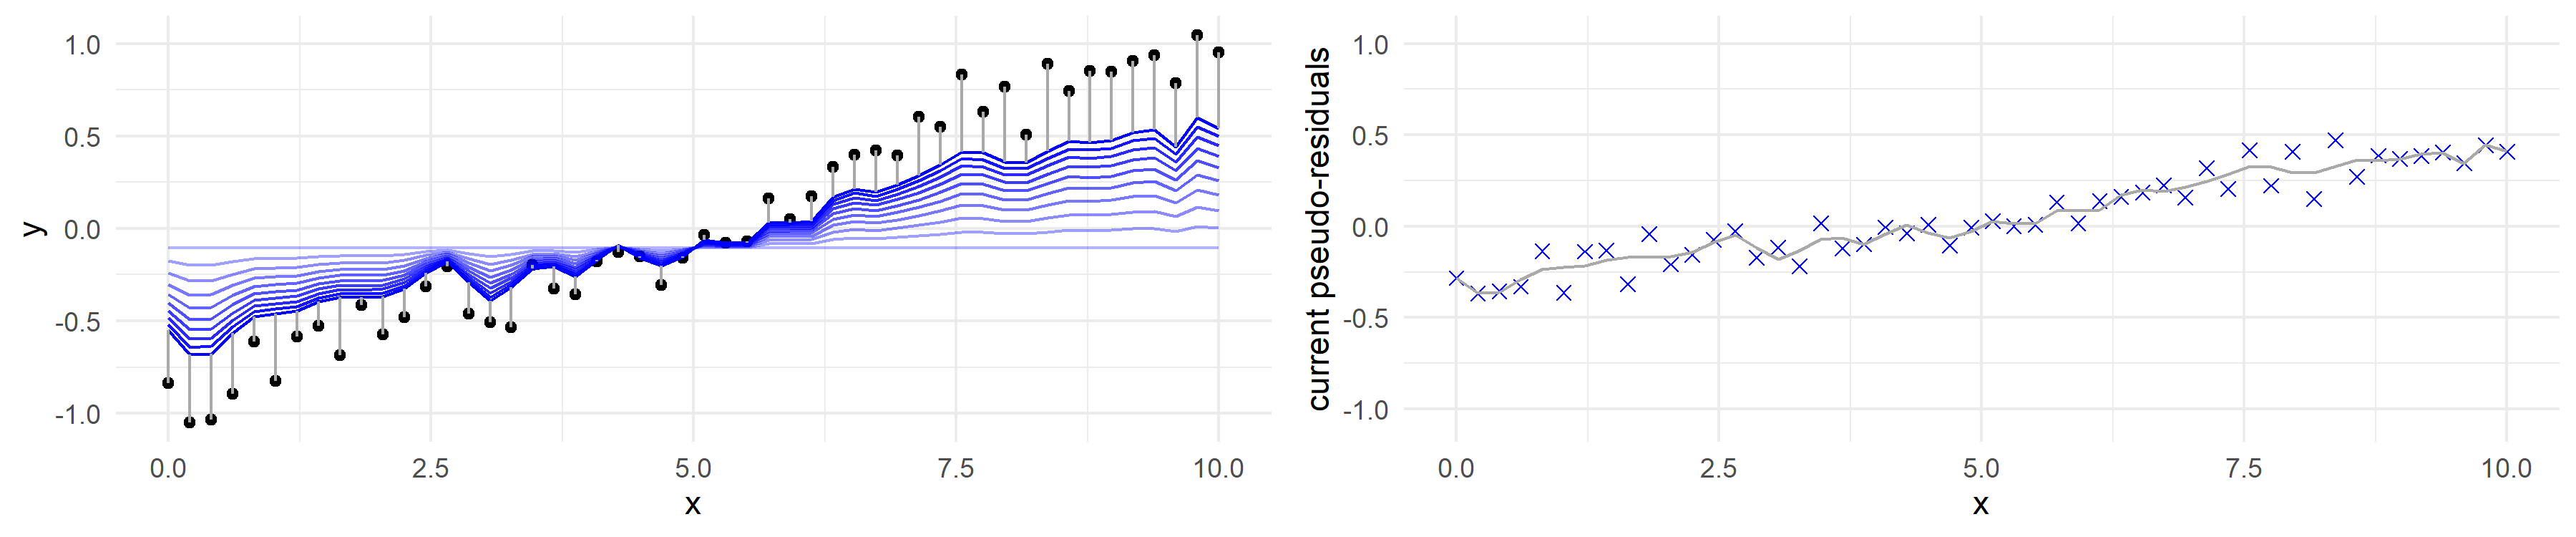
\includegraphics[width=\textwidth, trim=0 0 450 0, clip]{
  figure/illustration_gaussian_huber_2_10} \\
  \tiny{Boosting prediction function with GAM base learners for univariate 
  regression problem after 10 iterations}
\end{minipage}%
\hfill
\begin{minipage}{0.45\textwidth}
  % FIGURE SOURCE: http://arogozhnikov.github.io/2016/06/24/gradient_boosting_explained.html
  % 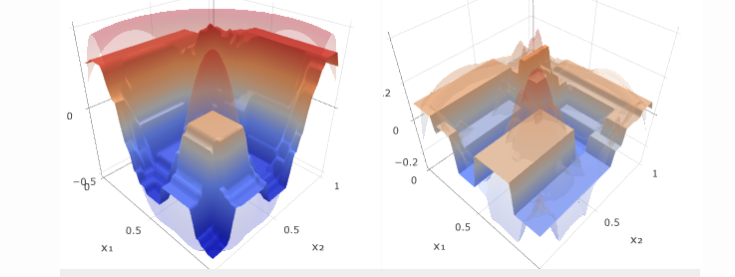
\includegraphics[width=\textwidth]{figure/gb-3d} \\
  \centering
  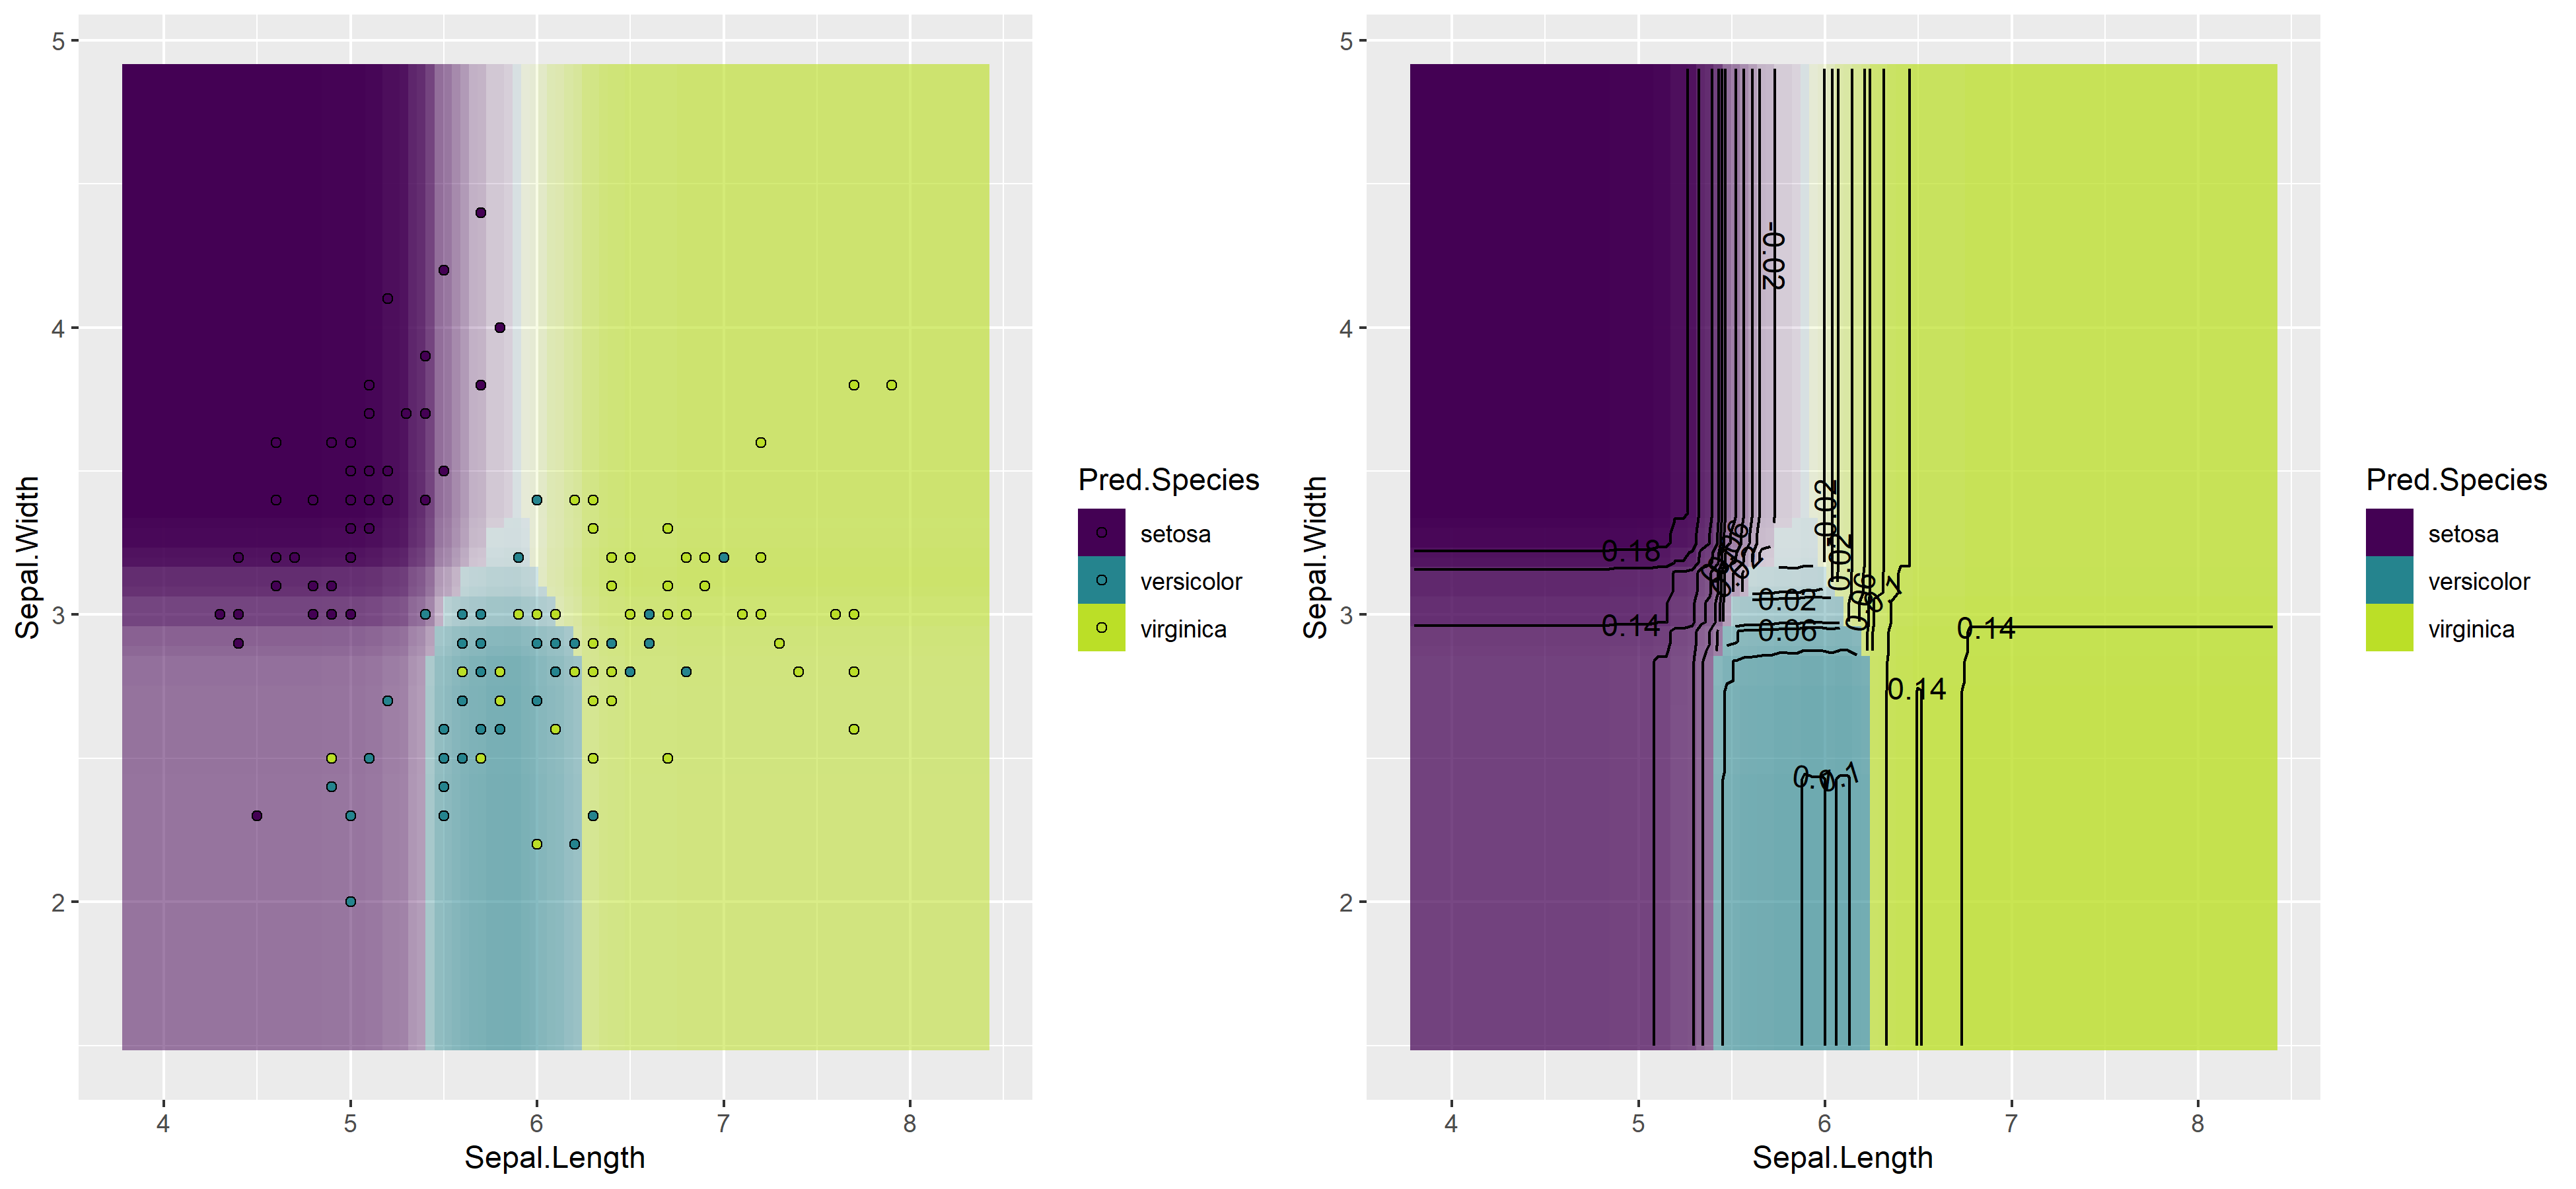
\includegraphics[width=\textwidth]{
  figure/boosting_multiclass_100} \\
  \tiny{Boosting prediction surface with tree base learners for \texttt{iris} 
  data after 100 iterations (\textit{right:} contour lines of discriminant 
  functions)}
\end{minipage}

\end{frame}

% ------------------------------------------------------------------------------

\begin{frame}{Gradient Boosting -- method summary}

\footnotesize

\highlight{Empirical risk}

\begin{itemize}
  \item In general, compatible with any \textbf{differentiable} loss
  \item Base learner in iteration $m$ is fitted on \textbf{Pseudo residuals}: \\
  $\tilde{r}^{(i)} = - \pd{\Lxyi}{\fxi}$ by minimizing the \textbf{L2-loss}: $\sumin (\tilde{r}^{(i)} - b(\xi, \bm{\theta}))^2$
\end{itemize}

\medskip

\highlight{Optimization} ~~
\begin{itemize}
    \item Same optimization procedure as base learner, while keeping the current ensemble $\fmdh$ fixed\\
    $\Rightarrow$ Efficient and generally applicable since \textit{inner} loss is always L2
    \item $\betam$ is found via \textbf{line search} or fixed to a \textbf{small constant value} and combined with the leaf values $\ctm$ for tree base learners: $\ctmt = \betam \cdot \ctm$
\end{itemize}

\medskip

\highlight{Hyperparameters}

\begin{itemize}
  \item \textbf{Ensemble size}, i.e., number of base learners
  \item \textbf{Complexity} of base learners (depending on type used)
  \item \textbf{Learning rate} $\beta$, i.e., impact of next base learner
\end{itemize}

\medskip

% \highlight{Runtime behavior} ~~ $\mathcal{O}(M \cdot n \cdot p)$ 
% for $M$ base learners, $n$ observations and $p$ features

\end{frame}


% ------------------------------------------------------------------------------

\begin{frame}{Gradient Boosting -- Practical hints}

\footnotesize

\highlight{Scalable Gradient Boosting} 

\begin{itemize}
  \item \textbf{Feature and data subsampling} for each base learner fit
  \item \textbf{Parallelization} and \textbf{approximate split finding} for tree base learners
  \item GPU accelaration
\end{itemize}

\medskip

\highlight{Explainable / Componentwise Gradient Boosting}
\begin{itemize}
    \item Base learners of \textbf{simple linear regression} models or \textbf{splines}, selecting a single feature in each iteration
    \item Allows \textbf{feature selection} and creates an \textbf{interpretable} model since uni- and bivariate effects can be visualized directly.
    \item Feature interactions can be learned via ranking techniques (e.g., GA$^2$M FAST)
\end{itemize}

\medskip

\highlight{Tuning}
\begin{itemize}
    \item Use \textbf{early-stopping} to determine ensemble size
    \item Various \textbf{regularization parameters}, e.g., L1/L2, number of leaves, ... that need to be carefully tuned
    \item Tune learning rate and base learner complexity hyperparameters on \textbf{log-scale}
\end{itemize}

\end{frame}

\begin{frame}{Gradient Boosting -- Implementation}

\highlight{Gradient Tree Boosting}
\begin{itemize}
  \item \textbf{R:} \texttt{mlr3} learners \texttt{LearnerClassifXgboost} / 
  \texttt{LearnerRegrXgboost}, \texttt{LearnerClassifLightGBM} / 
  \texttt{LearnerRegrLightGBM}
  \item \textbf{Python:} \texttt{GradientBoostingClassifier} / 
  \texttt{GradientBoostingRegressor} from package \texttt{scikit-learn}, 
  \texttt{XGBClassifier} / \texttt{XGBRegressor} from package \texttt{xgboost},
  \texttt{lgb.train} from package \texttt{lightgbm}
\end{itemize}

$\Rightarrow$ \texttt{LightGBM} current state-of-the-art but slightly more complicated to use than \texttt{xgboost} 

\medskip

\highlight{Componentwise Gradient Boosting}
\begin{itemize}
    \item \textbf{R:} \texttt{mboost} from package \texttt{mboost}, 
    \texttt{boostLinear} / \texttt{boostSplines} from package \texttt{compboost}
   \item \textbf{Python:} /
\end{itemize}

$\Rightarrow$ \texttt{mboost} very flexible but slow while \texttt{compboost} is much faster with limited features

\end{frame}


% ------------------------------------------------------------------------------

\begin{frame}{Gradient Boosting -- Pros \& Cons}

\footnotesize

\begin{columns}[onlytextwidth]
  \begin{column}{0.5\textwidth}
    \highlight{Advantages}
    \footnotesize
    \begin{itemize}
      \positem Retains of most of \textbf{base learners'} advantages 
      \positem Very \textbf{good predictor} due to aggressive loss minimization, typically only outperformed by heterogenous \textbf{stacking ensembles}
      \positem High \textbf{flexibility} via custom loss functions and choice of base learner
      \positem Highly efficient implementations exist (\texttt{lightgbm} / \texttt{xgboost}) that work well on large (distributed) data sets
      % \positem Applicable to \textbf{unbalanced} data
    \end{itemize}
  \end{column}
  \begin{column}{0.5\textwidth}
    \highlight{Disadvantages}
    \footnotesize
    \begin{itemize}
      \negitem Loss of base learners' potential \textbf{interpretability}
      \negitem \textbf{Many hyperparameters} 
      to be carefully tuned
      \negitem Hard to \textbf{parallelize} ($\rightsquigarrow$ solved by efficient implementation)
    \end{itemize}
  \end{column}
\end{columns}

\vfill

\small

\conclbox{High-performing and flexible predictor, but rather delicate to handle}

\end{frame}